\documentclass{standalone}
\usepackage{tikz}
\usetikzlibrary{patterns, positioning}
\usepackage[sfdefault]{ClearSans} %% option 'sfdefault' activates Clear Sans as the default text font
\usepackage[T1]{fontenc}

\begin{document}
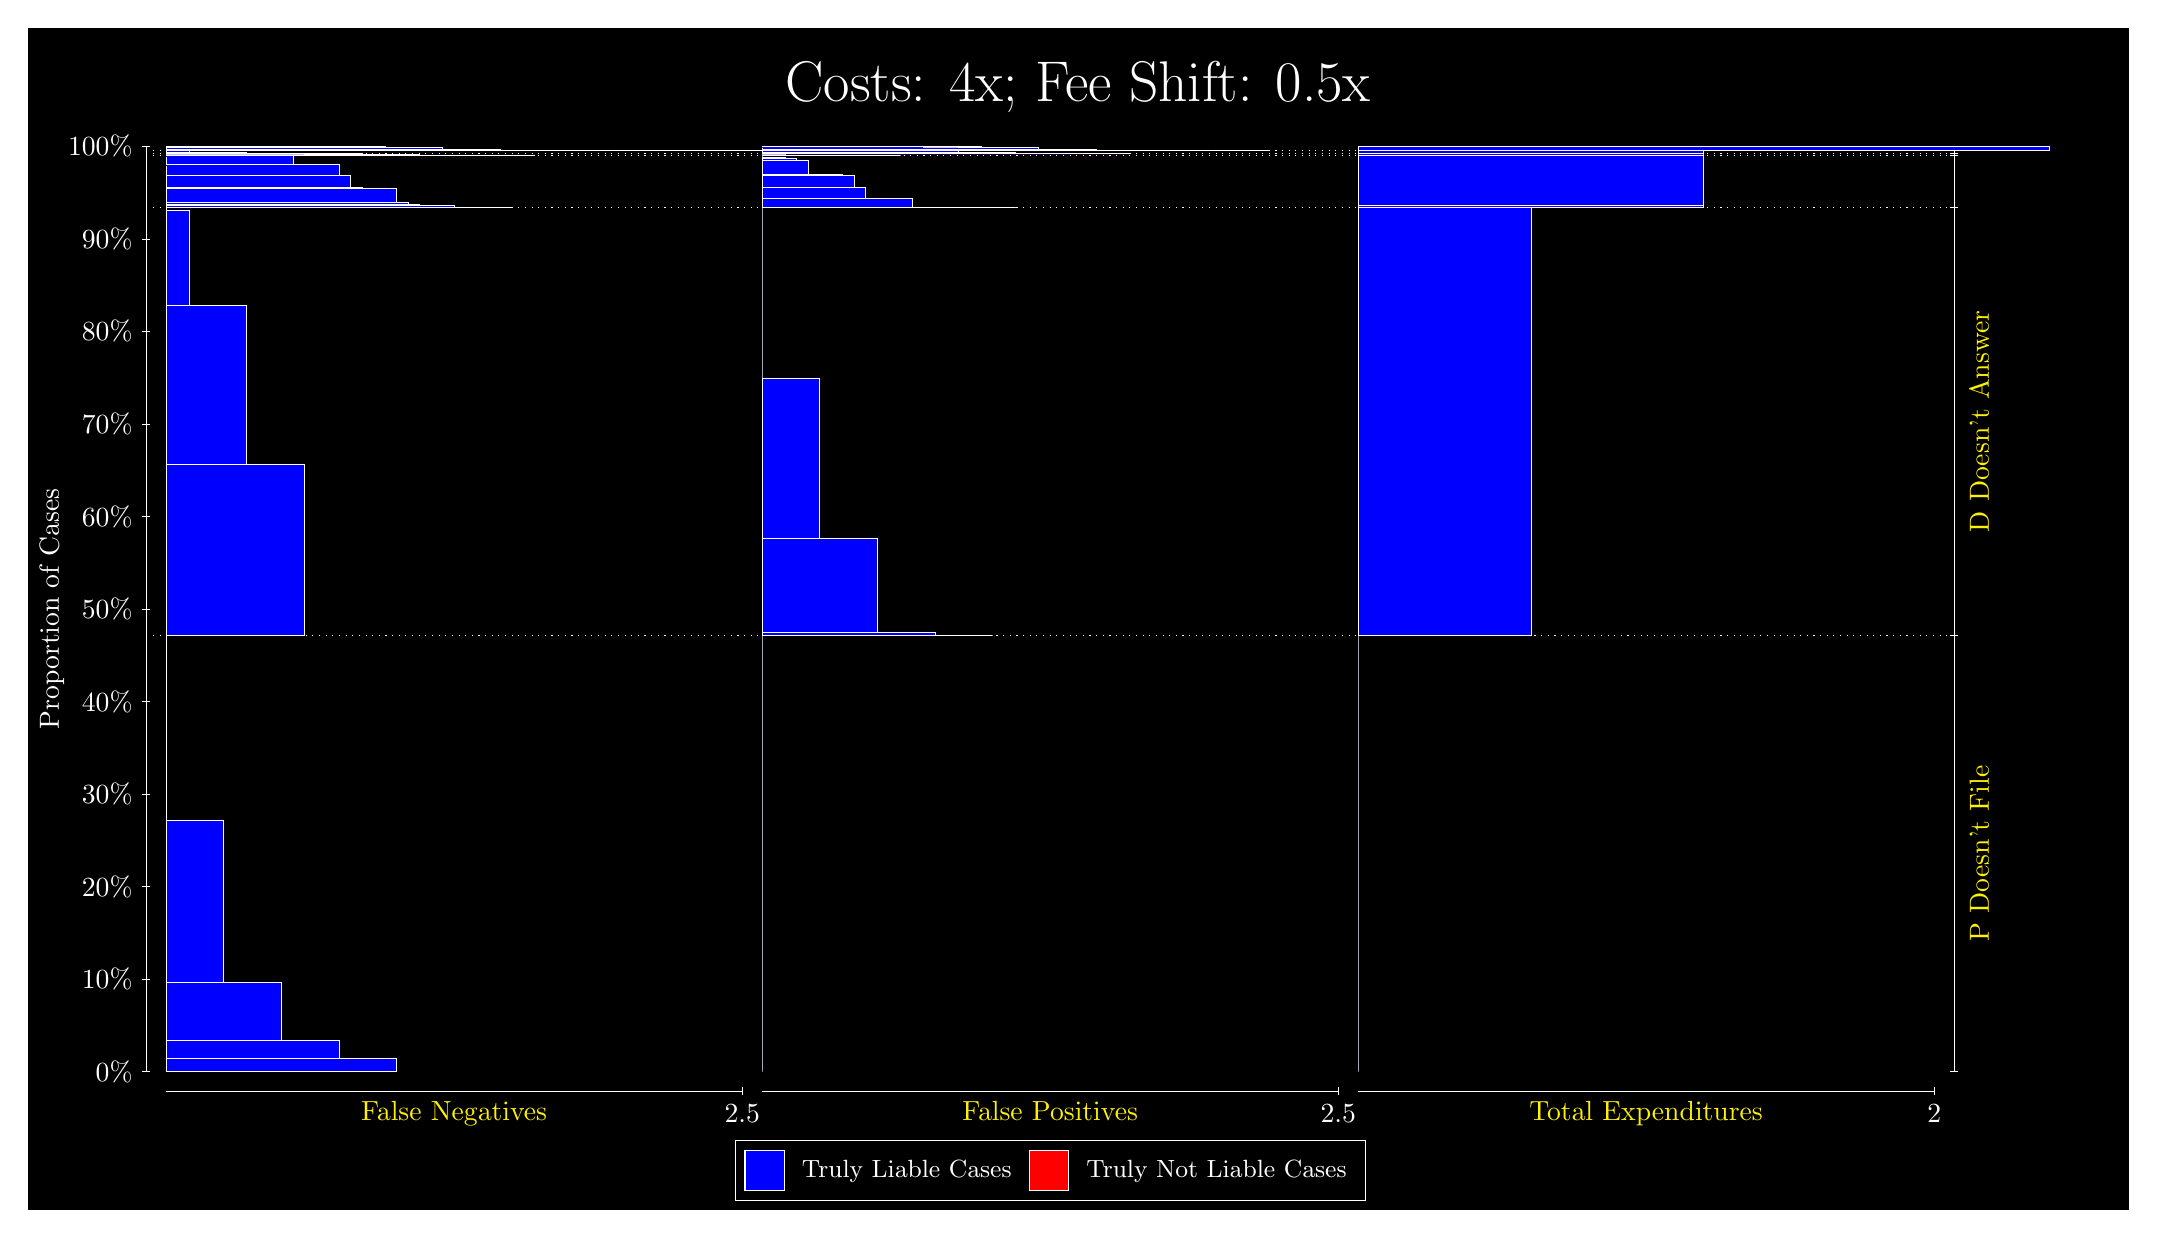
\begin{tikzpicture}
\draw[fill=black] (0,0) rectangle (26.667,15);
\draw[text=white] (0,13.5) rectangle (26.667,15) node[midway] {\huge Costs: 4x; Fee Shift: 0.5x};
\draw[white, very thin] (1.5,1.75) -- (1.5,13.5);
\node[rotate=90, text=white, anchor=center] at (0.3, 7.625) {Proportion of Cases};
\draw[white, very thin] (1.45,1.75) -- (1.55,1.75);
\node[text=white, anchor=east] at (1.45, 1.75) {0\%};
\draw[white, very thin] (1.45,2.925) -- (1.55,2.925);
\node[text=white, anchor=east] at (1.45, 2.925) {10\%};
\draw[white, very thin] (1.45,4.1) -- (1.55,4.1);
\node[text=white, anchor=east] at (1.45, 4.1) {20\%};
\draw[white, very thin] (1.45,5.275) -- (1.55,5.275);
\node[text=white, anchor=east] at (1.45, 5.275) {30\%};
\draw[white, very thin] (1.45,6.45) -- (1.55,6.45);
\node[text=white, anchor=east] at (1.45, 6.45) {40\%};
\draw[white, very thin] (1.45,7.625) -- (1.55,7.625);
\node[text=white, anchor=east] at (1.45, 7.625) {50\%};
\draw[white, very thin] (1.45,8.8) -- (1.55,8.8);
\node[text=white, anchor=east] at (1.45, 8.8) {60\%};
\draw[white, very thin] (1.45,9.975) -- (1.55,9.975);
\node[text=white, anchor=east] at (1.45, 9.975) {70\%};
\draw[white, very thin] (1.45,11.15) -- (1.55,11.15);
\node[text=white, anchor=east] at (1.45, 11.15) {80\%};
\draw[white, very thin] (1.45,12.325) -- (1.55,12.325);
\node[text=white, anchor=east] at (1.45, 12.325) {90\%};
\draw[white, very thin] (1.45,13.5) -- (1.55,13.5);
\node[text=white, anchor=east] at (1.45, 13.5) {100\%};

\draw[white, very thin] (24.457,1.75) -- (24.457,13.5);
\draw[white, very thin] (24.407,1.75) -- (24.507,1.75);
\node[anchor=west] at (24.407, 1.75) {};
\draw[white, very thin] (24.407,7.2886) -- (24.507,7.2886);
\node[anchor=west] at (24.407, 7.2886) {};
\draw[white, very thin] (24.407,12.726) -- (24.507,12.726);
\node[anchor=west] at (24.407, 12.726) {};
\draw[white, very thin] (24.407,13.385) -- (24.507,13.385);
\node[anchor=west] at (24.407, 13.385) {};
\draw[white, very thin] (24.407,13.407) -- (24.507,13.407);
\node[anchor=west] at (24.407, 13.407) {};
\draw[white, very thin] (24.407,13.447) -- (24.507,13.447);
\node[anchor=west] at (24.407, 13.447) {};
\draw[white, very thin] (24.407,13.5) -- (24.507,13.5);
\node[anchor=west] at (24.407, 13.5) {};

\draw[white, very thin, fill=blue] (1.75,1.75) rectangle (4.6775,1.9184);
\draw[white, very thin, fill=blue] (1.75,1.9184) rectangle (3.9457,2.1421);
\draw[white, very thin, fill=blue] (1.75,2.1421) rectangle (3.2138,2.8854);
\draw[white, very thin, fill=blue] (1.75,2.8854) rectangle (2.4819,4.9416);
\draw[white, very thin, fill=red] (1.75,4.9416) rectangle (1.75,4.9416);
\draw[white, very thin, fill=blue] (1.75,4.9416) rectangle (1.75,7.2886);
\draw[white, very thin, fill=blue] (1.75,7.2886) rectangle (3.5065,9.462);
\draw[white, very thin, fill=blue] (1.75,9.462) rectangle (2.7746,11.487);
\draw[white, very thin, fill=blue] (1.75,11.487) rectangle (2.0428,12.685);
\draw[white, very thin, fill=red] (1.75,12.685) rectangle (1.75,12.685);
\draw[white, very thin, fill=blue] (1.75,12.685) rectangle (1.75,12.726);
\draw[white, very thin, fill=blue] (1.75,12.726) rectangle (6.1413,12.726);
\draw[white, very thin, fill=blue] (1.75,12.726) rectangle (5.8486,12.726);
\draw[white, very thin, fill=blue] (1.75,12.726) rectangle (5.5558,12.727);
\draw[white, very thin, fill=blue] (1.75,12.727) rectangle (5.4094,12.75);
\draw[white, very thin, fill=blue] (1.75,12.75) rectangle (5.2631,12.75);
\draw[white, very thin, fill=blue] (1.75,12.75) rectangle (5.1167,12.752);
\draw[white, very thin, fill=blue] (1.75,12.752) rectangle (4.9703,12.758);
\draw[white, very thin, fill=blue] (1.75,12.758) rectangle (4.8239,12.784);
\draw[white, very thin, fill=blue] (1.75,12.784) rectangle (4.6775,12.966);
\draw[white, very thin, fill=blue] (1.75,12.966) rectangle (4.5312,12.967);
\draw[white, very thin, fill=blue] (1.75,12.967) rectangle (4.3848,12.969);
\draw[white, very thin, fill=blue] (1.75,12.969) rectangle (4.2384,12.981);
\draw[white, very thin, fill=blue] (1.75,12.981) rectangle (4.092,13.135);
\draw[white, very thin, fill=blue] (1.75,13.135) rectangle (3.9457,13.266);
\draw[white, very thin, fill=blue] (1.75,13.266) rectangle (3.7993,13.266);
\draw[white, very thin, fill=blue] (1.75,13.266) rectangle (3.6529,13.266);
\draw[white, very thin, fill=blue] (1.75,13.266) rectangle (3.5065,13.268);
\draw[white, very thin, fill=blue] (1.75,13.268) rectangle (3.3602,13.382);
\draw[white, very thin, fill=blue] (1.75,13.382) rectangle (3.2138,13.383);
\draw[white, very thin, fill=blue] (1.75,13.383) rectangle (3.0674,13.383);
\draw[white, very thin, fill=blue] (1.75,13.383) rectangle (2.921,13.383);
\draw[white, very thin, fill=blue] (1.75,13.383) rectangle (2.7746,13.383);
\draw[white, very thin, fill=blue] (1.75,13.383) rectangle (2.6283,13.385);
\draw[white, very thin, fill=blue] (1.75,13.385) rectangle (2.3355,13.385);
\draw[white, very thin, fill=blue] (1.75,13.385) rectangle (2.0428,13.385);
\draw[white, very thin, fill=red] (1.75,13.385) rectangle (1.75,13.385);
\draw[white, very thin, fill=blue] (1.75,13.385) rectangle (6.4341,13.385);
\draw[white, very thin, fill=blue] (1.75,13.385) rectangle (5.7022,13.389);
\draw[white, very thin, fill=blue] (1.75,13.389) rectangle (4.9703,13.401);
\draw[white, very thin, fill=blue] (1.75,13.401) rectangle (4.2384,13.407);
\draw[white, very thin, fill=blue] (1.75,13.407) rectangle (3.5065,13.407);
\draw[white, very thin, fill=red] (1.75,13.407) rectangle (1.75,13.407);
\draw[white, very thin, fill=blue] (1.75,13.407) rectangle (3.5065,13.407);
\draw[white, very thin, fill=blue] (1.75,13.407) rectangle (2.7746,13.429);
\draw[white, very thin, fill=blue] (1.75,13.429) rectangle (2.0428,13.446);
\draw[white, very thin, fill=red] (1.75,13.446) rectangle (1.75,13.446);
\draw[white, very thin, fill=blue] (1.75,13.446) rectangle (1.75,13.447);
\draw[white, very thin, fill=blue] (1.75,13.447) rectangle (9.9471,13.447);
\draw[white, very thin, fill=blue] (1.75,13.447) rectangle (9.2152,13.447);
\draw[white, very thin, fill=blue] (1.75,13.447) rectangle (8.4834,13.447);
\draw[white, very thin, fill=blue] (1.75,13.447) rectangle (7.7515,13.45);
\draw[white, very thin, fill=blue] (1.75,13.45) rectangle (7.4587,13.45);
\draw[white, very thin, fill=blue] (1.75,13.45) rectangle (7.0196,13.45);
\draw[white, very thin, fill=blue] (1.75,13.45) rectangle (6.7268,13.45);
\draw[white, very thin, fill=blue] (1.75,13.45) rectangle (6.2877,13.45);
\draw[white, very thin, fill=blue] (1.75,13.45) rectangle (5.9949,13.46);
\draw[white, very thin, fill=blue] (1.75,13.46) rectangle (5.2631,13.487);
\draw[white, very thin, fill=blue] (1.75,13.487) rectangle (4.5312,13.499);
\draw[white, very thin, fill=blue] (1.75,13.499) rectangle (3.7993,13.5);
\draw[white, very thin, fill=blue] (1.75,13.5) rectangle (3.0674,13.5);
\draw[white, very thin, fill=blue] (1.75,13.5) rectangle (2.3355,13.5);
\draw[white, very thin, fill=red] (1.75,13.5) rectangle (1.75,13.5);
\draw[white, very thin, fill=red] (9.3189,1.75) rectangle (9.3189,1.75);
\draw[white, very thin, fill=blue] (9.3189,1.75) rectangle (9.3189,7.2886);
\draw[white, very thin, fill=red] (9.3189,7.2886) rectangle (12.246,7.2886);
\draw[white, very thin, fill=blue] (9.3189,7.2886) rectangle (12.246,7.2886);
\draw[white, very thin, fill=blue] (9.3189,7.2886) rectangle (11.515,7.3302);
\draw[white, very thin, fill=blue] (9.3189,7.3302) rectangle (10.783,8.5282);
\draw[white, very thin, fill=blue] (9.3189,8.5282) rectangle (10.051,10.553);
\draw[white, very thin, fill=blue] (9.3189,10.553) rectangle (9.3189,12.726);
\draw[white, very thin, fill=red] (9.3189,12.726) rectangle (12.539,12.726);
\draw[white, very thin, fill=blue] (9.3189,12.726) rectangle (12.539,12.726);
\draw[white, very thin, fill=red] (9.3189,12.726) rectangle (12.246,12.726);
\draw[white, very thin, fill=blue] (9.3189,12.726) rectangle (12.246,12.726);
\draw[white, very thin, fill=red] (9.3189,12.726) rectangle (11.954,12.726);
\draw[white, very thin, fill=blue] (9.3189,12.726) rectangle (11.954,12.728);
\draw[white, very thin, fill=blue] (9.3189,12.728) rectangle (11.807,12.728);
\draw[white, very thin, fill=red] (9.3189,12.728) rectangle (11.661,12.728);
\draw[white, very thin, fill=blue] (9.3189,12.728) rectangle (11.661,12.728);
\draw[white, very thin, fill=blue] (9.3189,12.728) rectangle (11.515,12.728);
\draw[white, very thin, fill=red] (9.3189,12.728) rectangle (11.368,12.728);
\draw[white, very thin, fill=blue] (9.3189,12.728) rectangle (11.368,12.729);
\draw[white, very thin, fill=blue] (9.3189,12.729) rectangle (11.222,12.843);
\draw[white, very thin, fill=blue] (9.3189,12.843) rectangle (11.075,12.845);
\draw[white, very thin, fill=blue] (9.3189,12.845) rectangle (10.929,12.845);
\draw[white, very thin, fill=blue] (9.3189,12.845) rectangle (10.783,12.845);
\draw[white, very thin, fill=blue] (9.3189,12.845) rectangle (10.636,12.976);
\draw[white, very thin, fill=blue] (9.3189,12.976) rectangle (10.49,13.13);
\draw[white, very thin, fill=blue] (9.3189,13.13) rectangle (10.344,13.142);
\draw[white, very thin, fill=blue] (9.3189,13.142) rectangle (10.197,13.144);
\draw[white, very thin, fill=blue] (9.3189,13.144) rectangle (10.051,13.145);
\draw[white, very thin, fill=blue] (9.3189,13.145) rectangle (9.9044,13.327);
\draw[white, very thin, fill=blue] (9.3189,13.327) rectangle (9.758,13.353);
\draw[white, very thin, fill=blue] (9.3189,13.353) rectangle (9.6116,13.359);
\draw[white, very thin, fill=blue] (9.3189,13.359) rectangle (9.4652,13.361);
\draw[white, very thin, fill=blue] (9.3189,13.361) rectangle (9.3189,13.385);
\draw[white, very thin, fill=red] (9.3189,13.385) rectangle (11.075,13.385);
\draw[white, very thin, fill=blue] (9.3189,13.385) rectangle (11.075,13.385);
\draw[white, very thin, fill=blue] (9.3189,13.385) rectangle (10.344,13.391);
\draw[white, very thin, fill=blue] (9.3189,13.391) rectangle (9.6116,13.402);
\draw[white, very thin, fill=blue] (9.3189,13.402) rectangle (9.3189,13.407);
\draw[white, very thin, fill=red] (9.3189,13.407) rectangle (14.003,13.407);
\draw[white, very thin, fill=blue] (9.3189,13.407) rectangle (14.003,13.407);
\draw[white, very thin, fill=blue] (9.3189,13.407) rectangle (13.271,13.407);
\draw[white, very thin, fill=blue] (9.3189,13.407) rectangle (12.539,13.425);
\draw[white, very thin, fill=blue] (9.3189,13.425) rectangle (11.807,13.446);
\draw[white, very thin, fill=blue] (9.3189,13.446) rectangle (11.075,13.447);
\draw[white, very thin, fill=red] (9.3189,13.447) rectangle (15.759,13.447);
\draw[white, very thin, fill=blue] (9.3189,13.447) rectangle (15.759,13.447);
\draw[white, very thin, fill=blue] (9.3189,13.447) rectangle (15.028,13.447);
\draw[white, very thin, fill=red] (9.3189,13.447) rectangle (15.028,13.447);
\draw[white, very thin, fill=blue] (9.3189,13.447) rectangle (15.028,13.447);
\draw[white, very thin, fill=blue] (9.3189,13.447) rectangle (14.296,13.447);
\draw[white, very thin, fill=red] (9.3189,13.447) rectangle (14.296,13.447);
\draw[white, very thin, fill=blue] (9.3189,13.447) rectangle (14.296,13.447);
\draw[white, very thin, fill=blue] (9.3189,13.447) rectangle (13.564,13.45);
\draw[white, very thin, fill=red] (9.3189,13.45) rectangle (13.564,13.45);
\draw[white, very thin, fill=blue] (9.3189,13.45) rectangle (13.564,13.46);
\draw[white, very thin, fill=blue] (9.3189,13.46) rectangle (12.832,13.46);
\draw[white, very thin, fill=blue] (9.3189,13.46) rectangle (12.832,13.486);
\draw[white, very thin, fill=blue] (9.3189,13.486) rectangle (12.1,13.496);
\draw[white, very thin, fill=red] (9.3189,13.496) rectangle (11.807,13.496);
\draw[white, very thin, fill=blue] (9.3189,13.496) rectangle (11.807,13.496);
\draw[white, very thin, fill=blue] (9.3189,13.496) rectangle (11.368,13.497);
\draw[white, very thin, fill=red] (9.3189,13.497) rectangle (11.075,13.497);
\draw[white, very thin, fill=blue] (9.3189,13.497) rectangle (11.075,13.497);
\draw[white, very thin, fill=blue] (9.3189,13.497) rectangle (10.636,13.497);
\draw[white, very thin, fill=blue] (9.3189,13.497) rectangle (10.344,13.499);
\draw[white, very thin, fill=blue] (9.3189,13.499) rectangle (9.6116,13.5);
\draw[white, very thin, fill=blue] (9.3189,13.5) rectangle (9.3189,13.5);
\draw[white, very thin, fill=red] (16.888,1.75) rectangle (16.888,1.75);
\draw[white, very thin, fill=blue] (16.888,1.75) rectangle (16.888,7.2886);
\draw[white, very thin, fill=red] (16.888,7.2886) rectangle (19.083,7.2886);
\draw[white, very thin, fill=blue] (16.888,7.2886) rectangle (19.083,12.726);
\draw[white, very thin, fill=red] (16.888,12.726) rectangle (21.279,12.726);
\draw[white, very thin, fill=blue] (16.888,12.726) rectangle (21.279,12.746);
\draw[white, very thin, fill=red] (16.888,12.746) rectangle (21.279,12.746);
\draw[white, very thin, fill=blue] (16.888,12.746) rectangle (21.279,13.385);
\draw[white, very thin, fill=red] (16.888,13.385) rectangle (21.279,13.385);
\draw[white, very thin, fill=blue] (16.888,13.385) rectangle (21.279,13.407);
\draw[white, very thin, fill=red] (16.888,13.407) rectangle (21.279,13.407);
\draw[white, very thin, fill=blue] (16.888,13.407) rectangle (21.279,13.447);
\draw[white, very thin, fill=red] (16.888,13.447) rectangle (25.67,13.447);
\draw[white, very thin, fill=blue] (16.888,13.447) rectangle (25.67,13.451);
\draw[white, very thin, fill=red] (16.888,13.451) rectangle (25.67,13.451);
\draw[white, very thin, fill=blue] (16.888,13.451) rectangle (25.67,13.5);
\draw[white, dotted] (1.5,7.2886) -- (24.457,7.2886);
\draw[white, dotted] (1.5,12.726) -- (24.457,12.726);
\draw[white, dotted] (1.5,13.385) -- (24.457,13.385);
\draw[white, dotted] (1.5,13.407) -- (24.457,13.407);
\draw[white, dotted] (1.5,13.447) -- (24.457,13.447);
\draw[white, very thin] (1.75,1.5) -- (9.0689,1.5);
\node[text=yellow, anchor=north] at (5.4094, 1.5) {False Negatives};
\draw[white, very thin] (9.0689,1.45) -- (9.0689,1.55);
\node[text=white, anchor=north] at (9.0689, 1.45) {2.5};

\draw[white, very thin] (9.3189,1.5) -- (16.638,1.5);
\node[text=yellow, anchor=north] at (12.978, 1.5) {False Positives};
\draw[white, very thin] (16.638,1.45) -- (16.638,1.55);
\node[text=white, anchor=north] at (16.638, 1.45) {2.5};

\draw[white, very thin] (16.888,1.5) -- (24.207,1.5);
\node[text=yellow, anchor=north] at (20.547, 1.5) {Total Expenditures};
\draw[white, very thin] (24.207,1.45) -- (24.207,1.55);
\node[text=white, anchor=north] at (24.207, 1.45) {2};

\node[text=yellow, centered, rotate=90] at (24.777, 4.5193) {P Doesn't File};
\node[text=yellow, centered, rotate=90] at (24.777, 10.007) {D Doesn't Answer};





\draw (12.978300999999998,1.5) node[draw=none] (baseCoordinate) {};
\begin{scope}[align=center]
        \matrix[scale=0.5, draw=white, below=0.5cm of baseCoordinate, nodes={draw}, column sep=0.1cm]{
            \node[rectangle, draw, minimum width=0.5cm, minimum height=0.5cm, fill=blue] {}; &
            \node[draw=none, font=\small, text=white] (B) {Truly Liable Cases}; &
            \node[rectangle, draw, minimum width=0.5cm, minimum height=0.5cm, fill=red] {}; &
            \node[draw=none, font=\small, text=white] (B) {Truly Not Liable Cases}; \\
            };
\end{scope}

\end{tikzpicture}
\end{document}